\documentclass[nooutcomes]{ximera}
%handout:  for handout version with no solutions or instructor notes
%handout,instructornotes:  for instructor version with just problems and notes, no solutions
%noinstructornotes:  shows only problem and solutions

%% handout
%% space
%% newpage
%% numbers
%% nooutcomes



%\begin{image}
%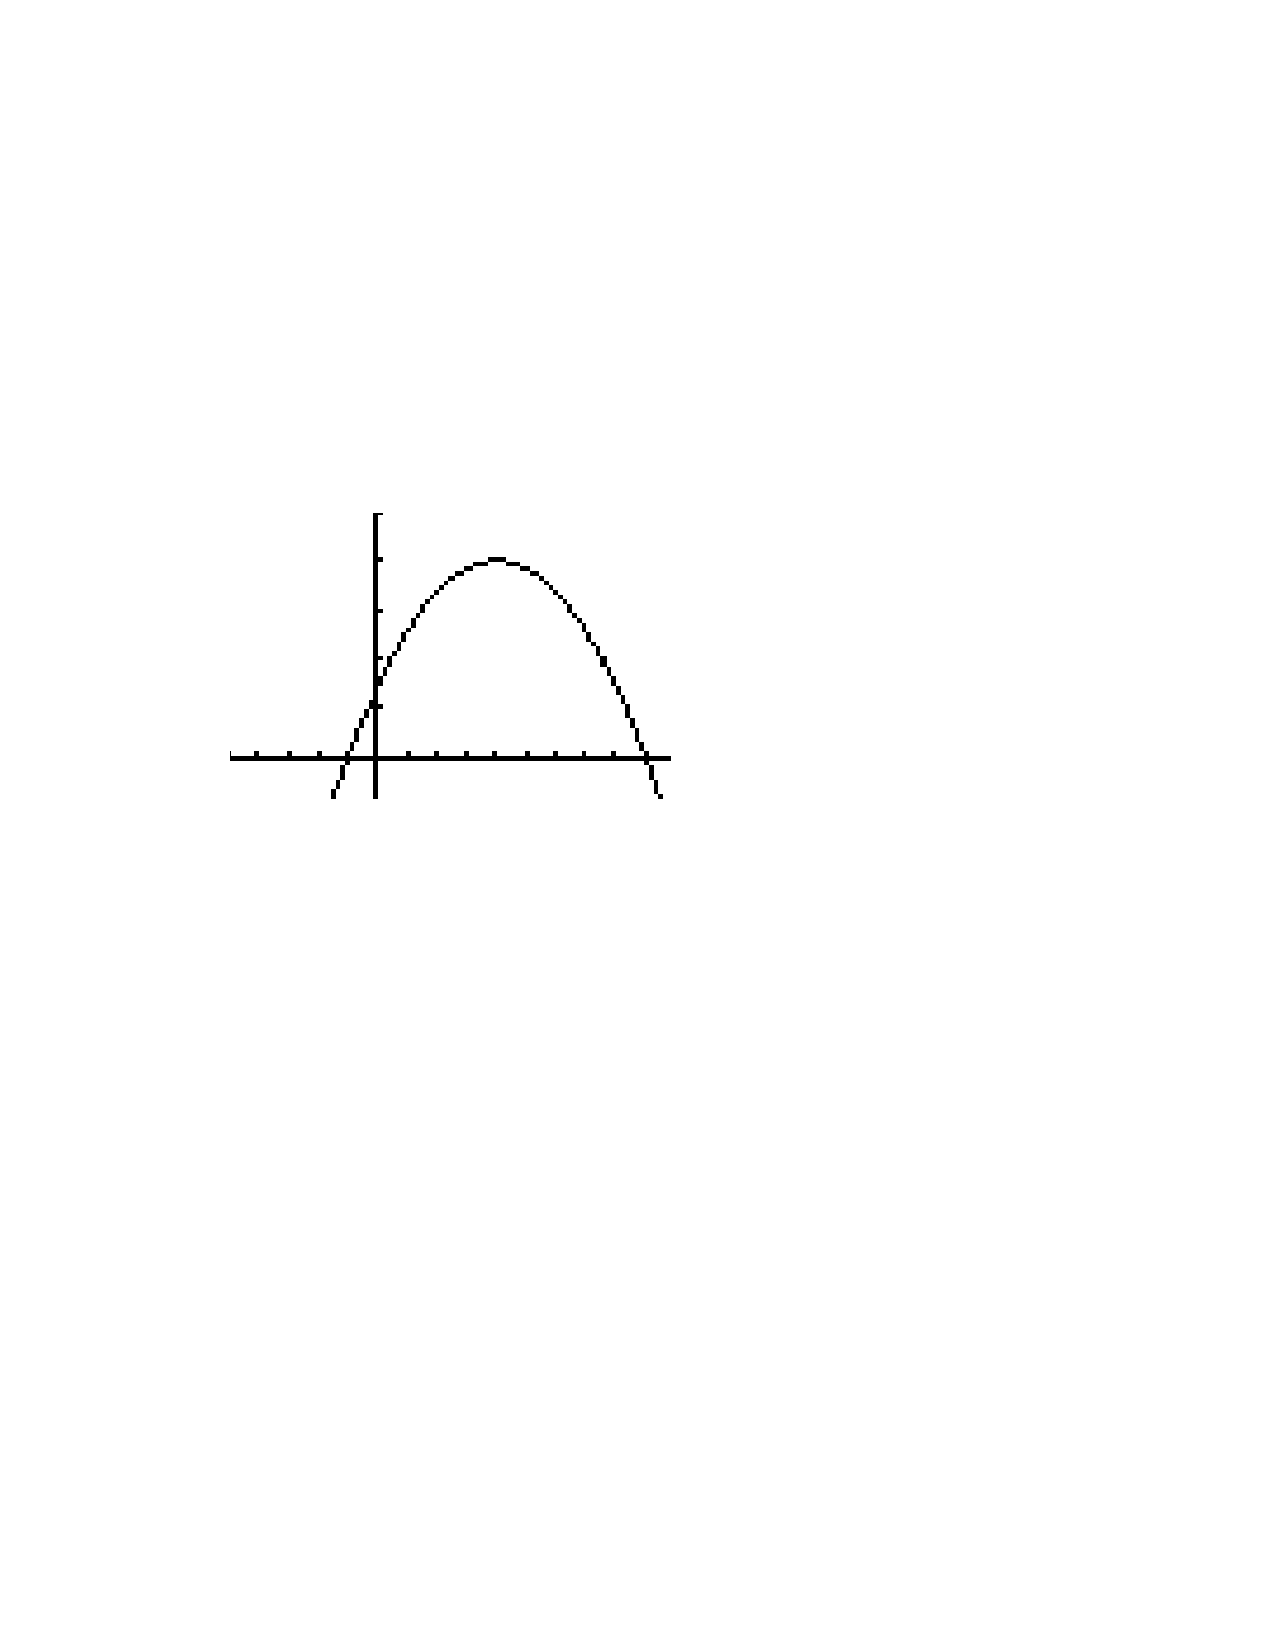
\includegraphics{Figure1.pdf}
%\end{image}

%add a ``.'' below when used in a specific directory.
\newcommand{\RR}{\mathbb R}
\renewcommand{\d}{\,d}
\newcommand{\dd}[2][]{\frac{d #1}{d #2}}
\renewcommand{\l}{\ell}
\newcommand{\ddx}{\frac{d}{dx}}
\newcommand{\dfn}{\textbf}
\newcommand{\eval}[1]{\bigg[ #1 \bigg]}

\usepackage{multicol}

\renewenvironment{freeResponse}{
\ifhandout\setbox0\vbox\bgroup\else
\begin{trivlist}\item[\hskip \labelsep\bfseries Solution:\hspace{2ex}]
\fi}
{\ifhandout\egroup\else
\end{trivlist}
\fi} %% we can turn off input when making a master document

\usepackage{fullpage}

\title{1.1 and 1.2:  Review of Functions}  

\begin{document}
\begin{abstract}		\end{abstract}
\maketitle


%problem 1
\begin{problem}
Define 
	$f(x) =   \left\{ \begin{array}{cl}
	x^2-1		 	&	\qquad \text{if } x < 0					\\
	\text{? }			&	\qquad \text{if }  x > 0 	\\		\end{array} \right.  $
\begin{enumerate}	
	\item  Find an expression for "?" such that $f$ will be even.
	
	\begin{freeResponse} 
			If $f$ is even then $f(x)=f(-x)$.  
			\begin{align*}
			f(x)&=f(-x)\ \text{for}\ x>0\\
			&=(-x)^2-1\\
			&=x^2-1	
			\end{align*}

	\begin{image}		
	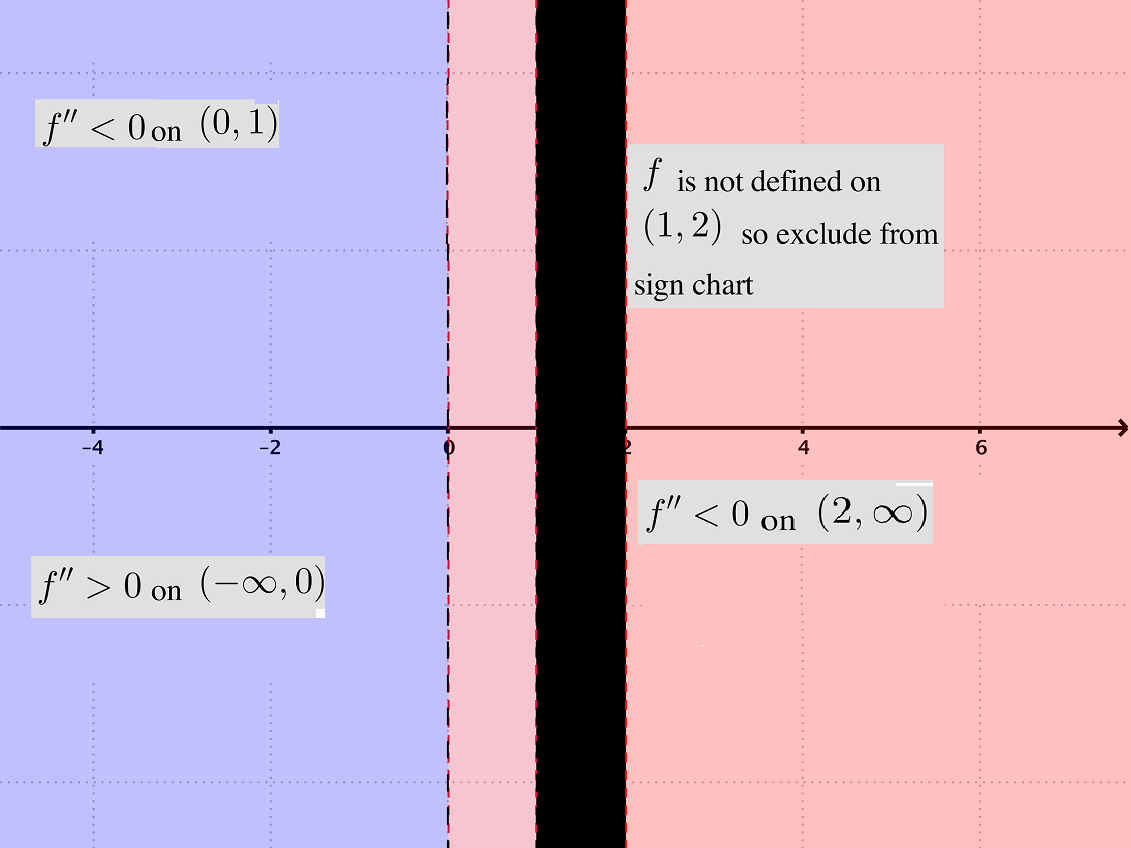
\includegraphics[scale=.4]{figure11.png}
	\end{image}
		
	\end{freeResponse}
	
	\item  Find an expression for "?" such that $f$ will be odd.
	
	\begin{freeResponse}
	   If $f$ is odd then $f(-x)=-f(x)$. 
			\begin{align*}
			-f(x)&=f(-x)\ \text{for}\ x>0\\
			&=(-x)^2-1\\
			&=x^2-1\\
			& \implies f(x)=-x^2+1	
			\end{align*}
	
	\begin{image}		
	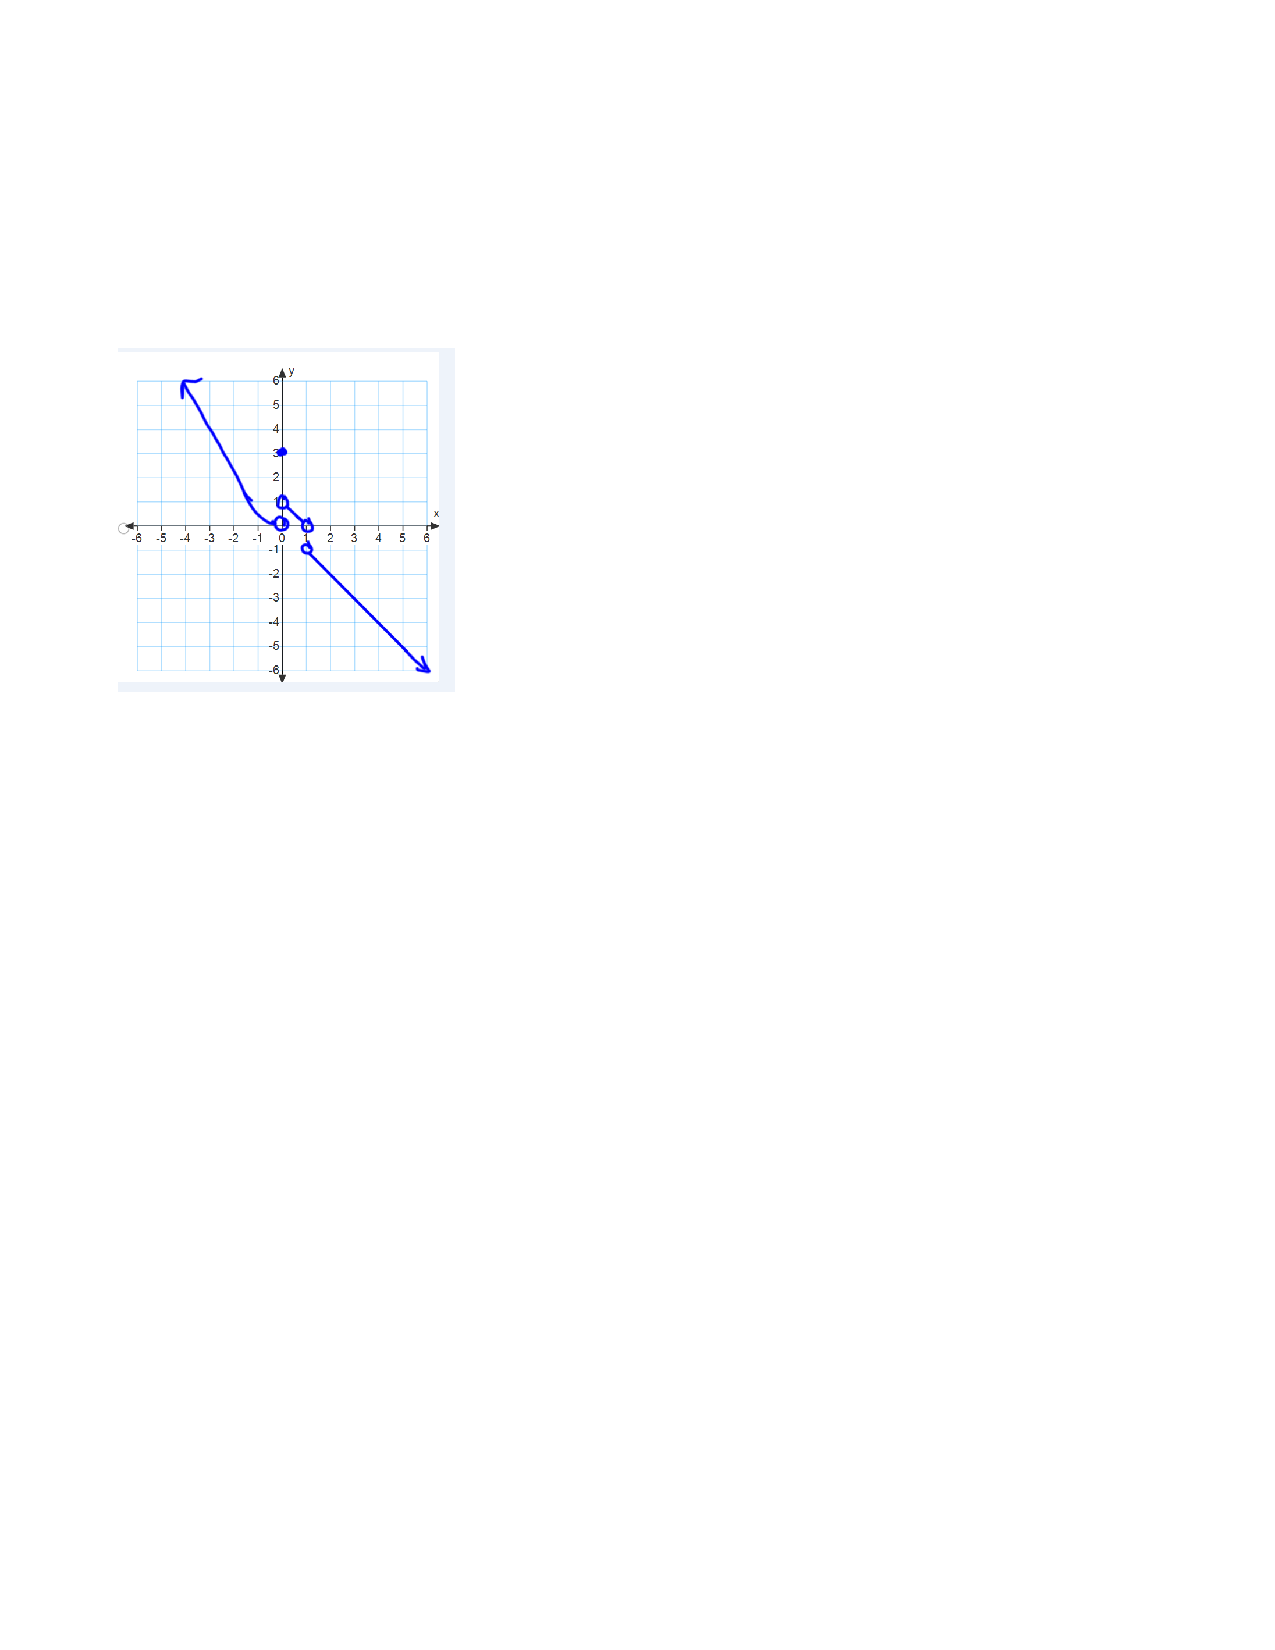
\includegraphics[scale=.5]{Figure3.png}
	\end{image}
		

	\end{freeResponse}


	\end{enumerate}
	
	
	
	
\end{problem}




%problem 2
\begin{problem}
The graph of $g(x)=e^x$ is given below.

	\begin{image}		
	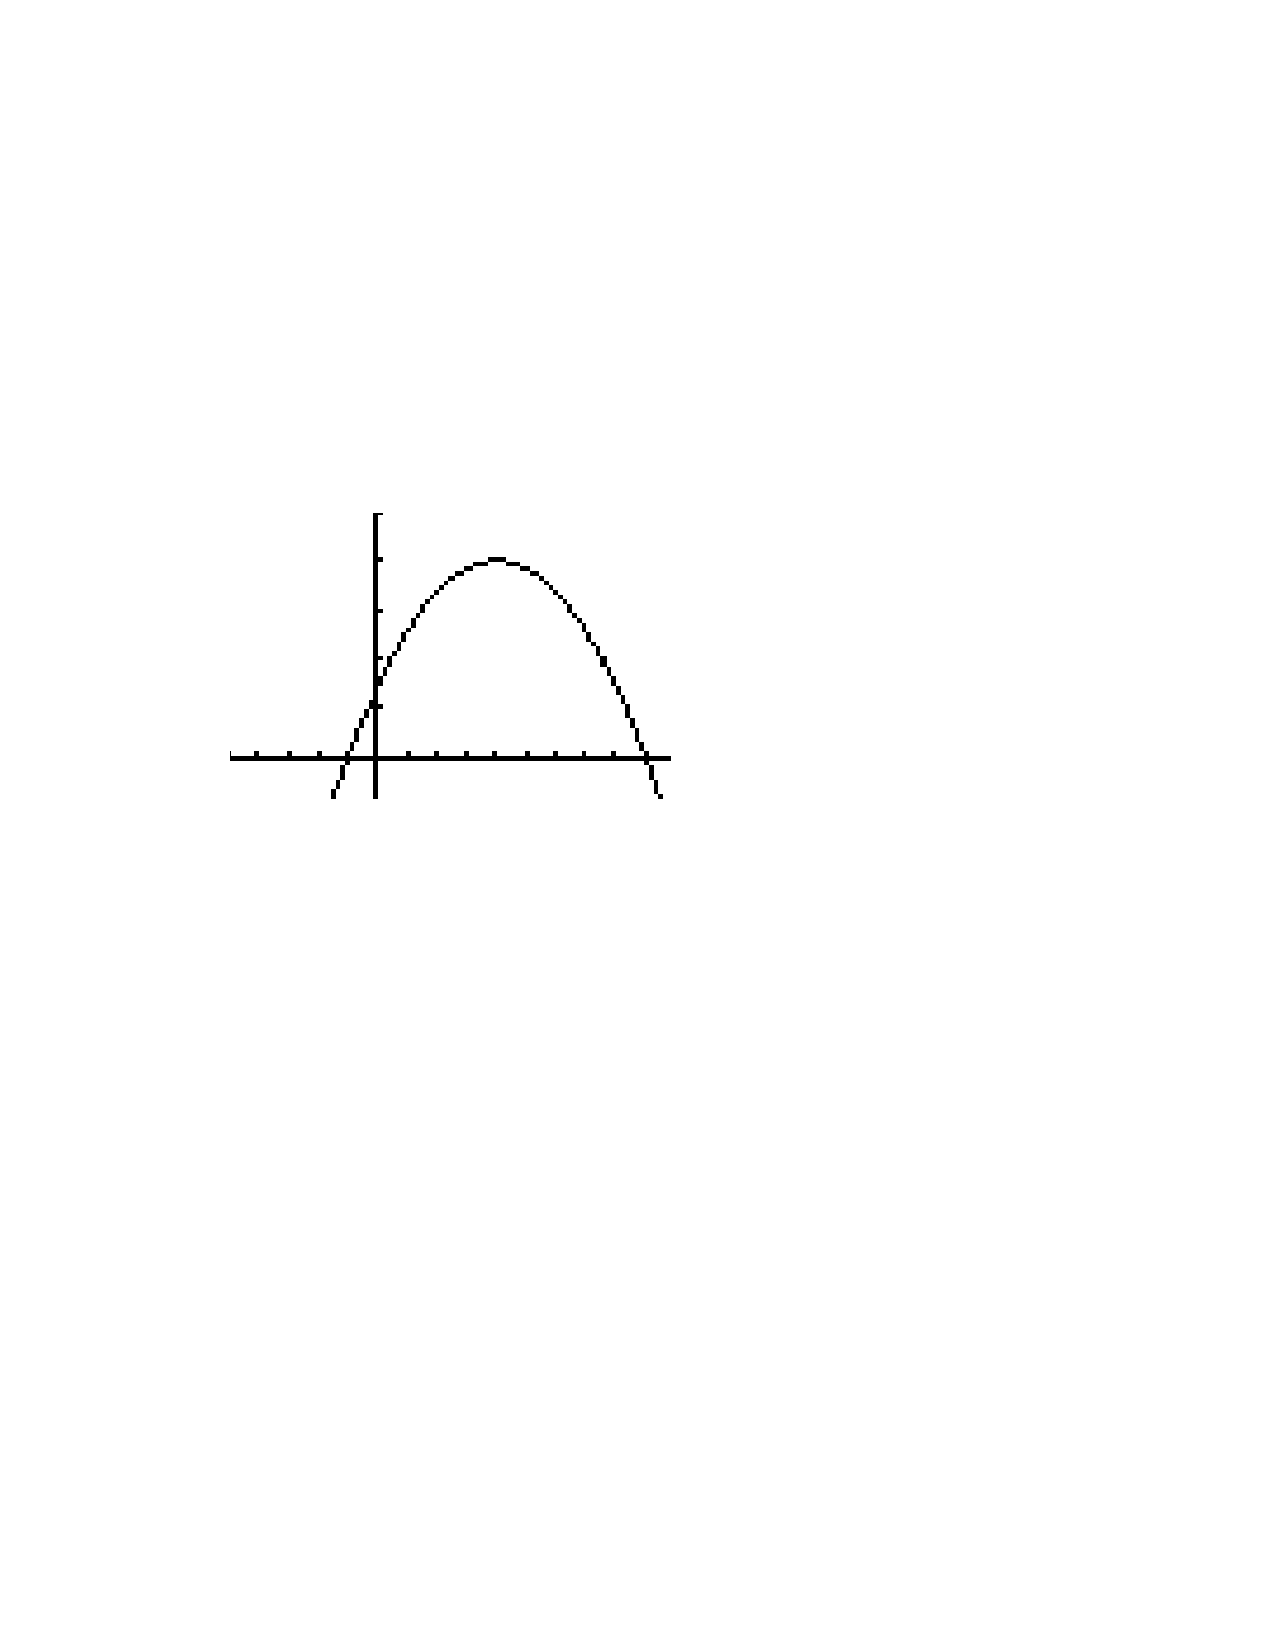
\includegraphics[scale=.6]{Figure1.pdf}
	\end{image}

\begin{enumerate}	
	\item  Find the domain and range of $g$.
		\begin{freeResponse}
		Domain: $(-\infty,\infty)$, Range: $(0,\infty)$
		\end{freeResponse}


	
	\item  Find the values of $g(1), g(0), g(-1)$ and plot the points $(1,g(1)), (0,g(0)),$ and $(-1,g(-1))$  on the graph below.
		\begin{freeResponse}
	
			$$g(1)=e^1=e$$
			$$ g(0)=e^0=1$$ 
			$$g(-1)=e^{-1}=\frac{1}{e}$$
			 These are values of $g(x)=e^x$ that you should know.

		\begin{image}		
		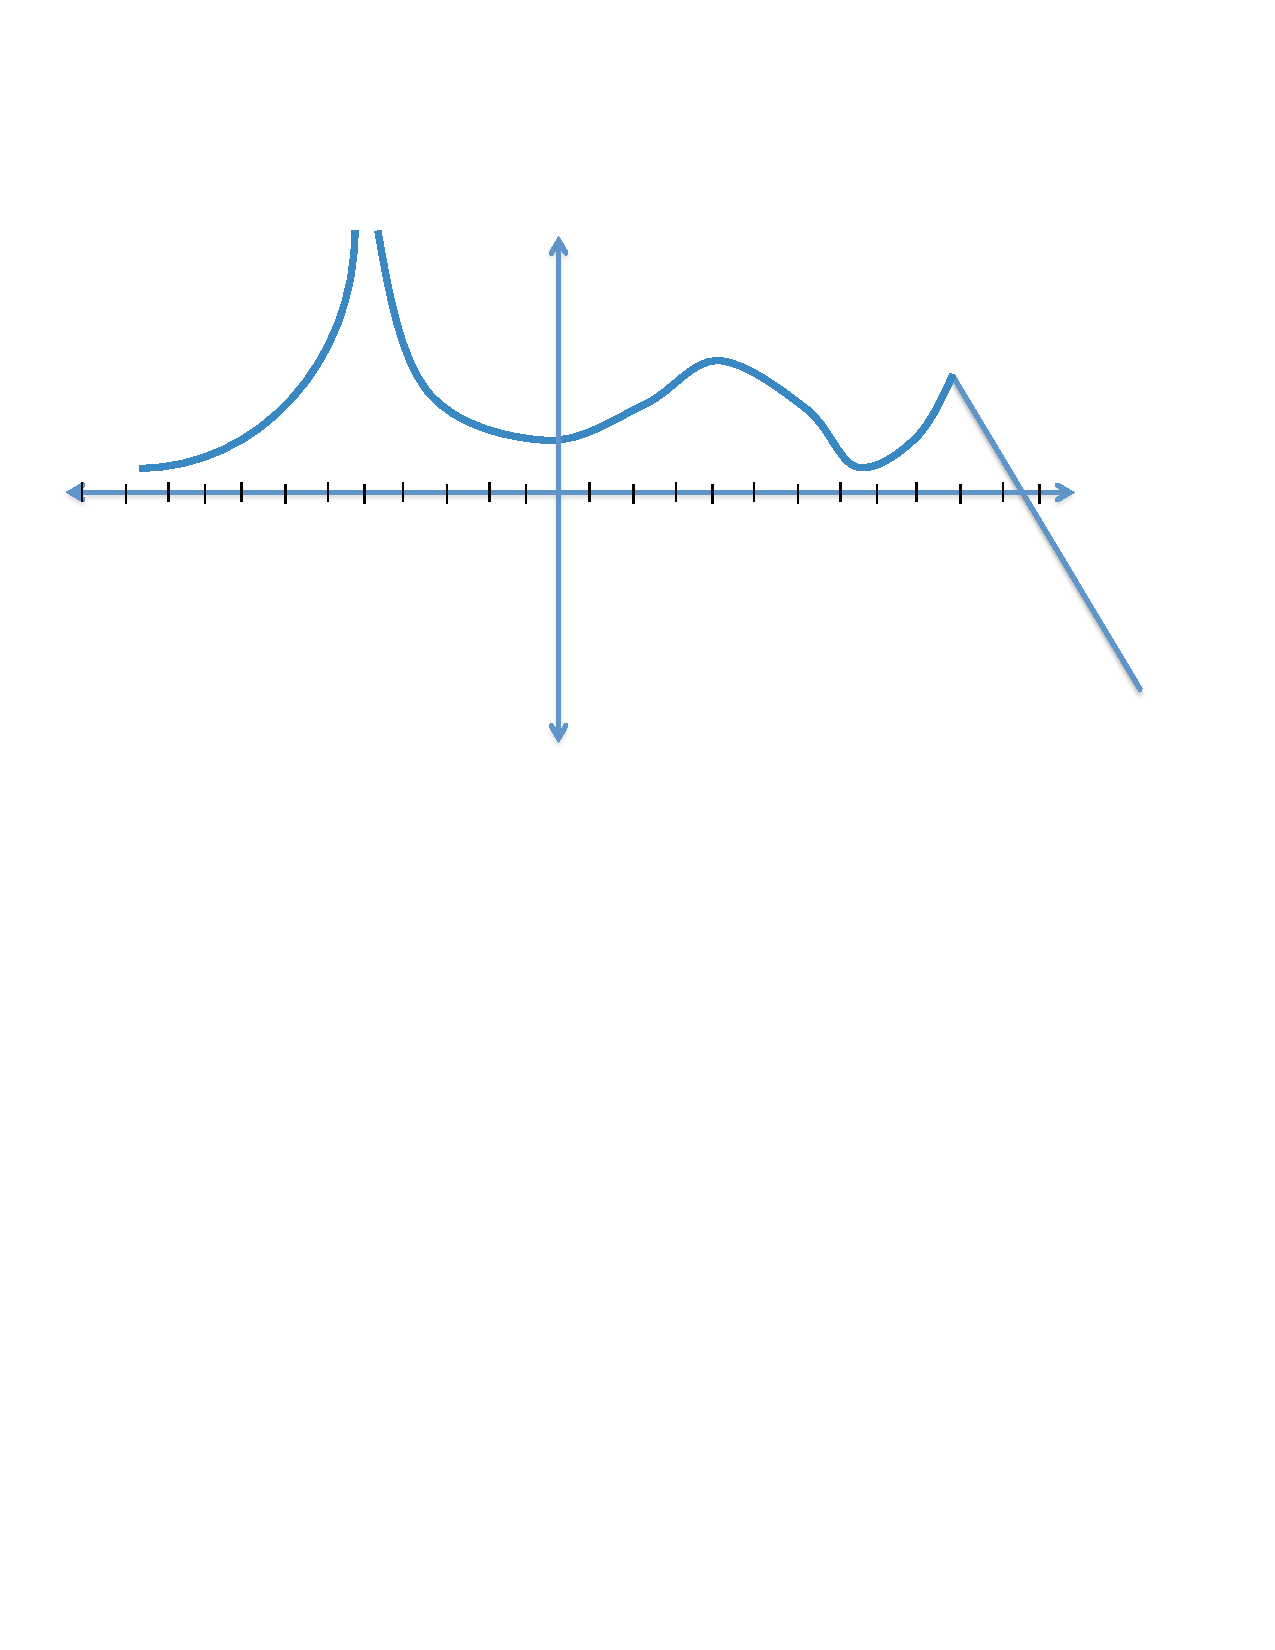
\includegraphics[scale=.6]{Figure5.pdf}
		\end{image}


		\end{freeResponse}
	\item Graph $h(x)=ln(x)$ on the same axis below.
		\begin{freeResponse}
		Recall:  $ln(x)$ is the inverse of $e^x$.  To find the graph of $ln(x)$ we reflect the graph of $e^x$ over the line $y=x$.  Since the points $\left(-1,\frac{1}{e}\right),(0,1),(1,e)$ are on $y=e^x=g(x)$, the points $\left(\frac{1}{e}, -1\right),(1,0),(e,1)$ are on the graph of $y=\ln(x)=g^{-1}(x)=h(x)$ 

		\begin{image}		
		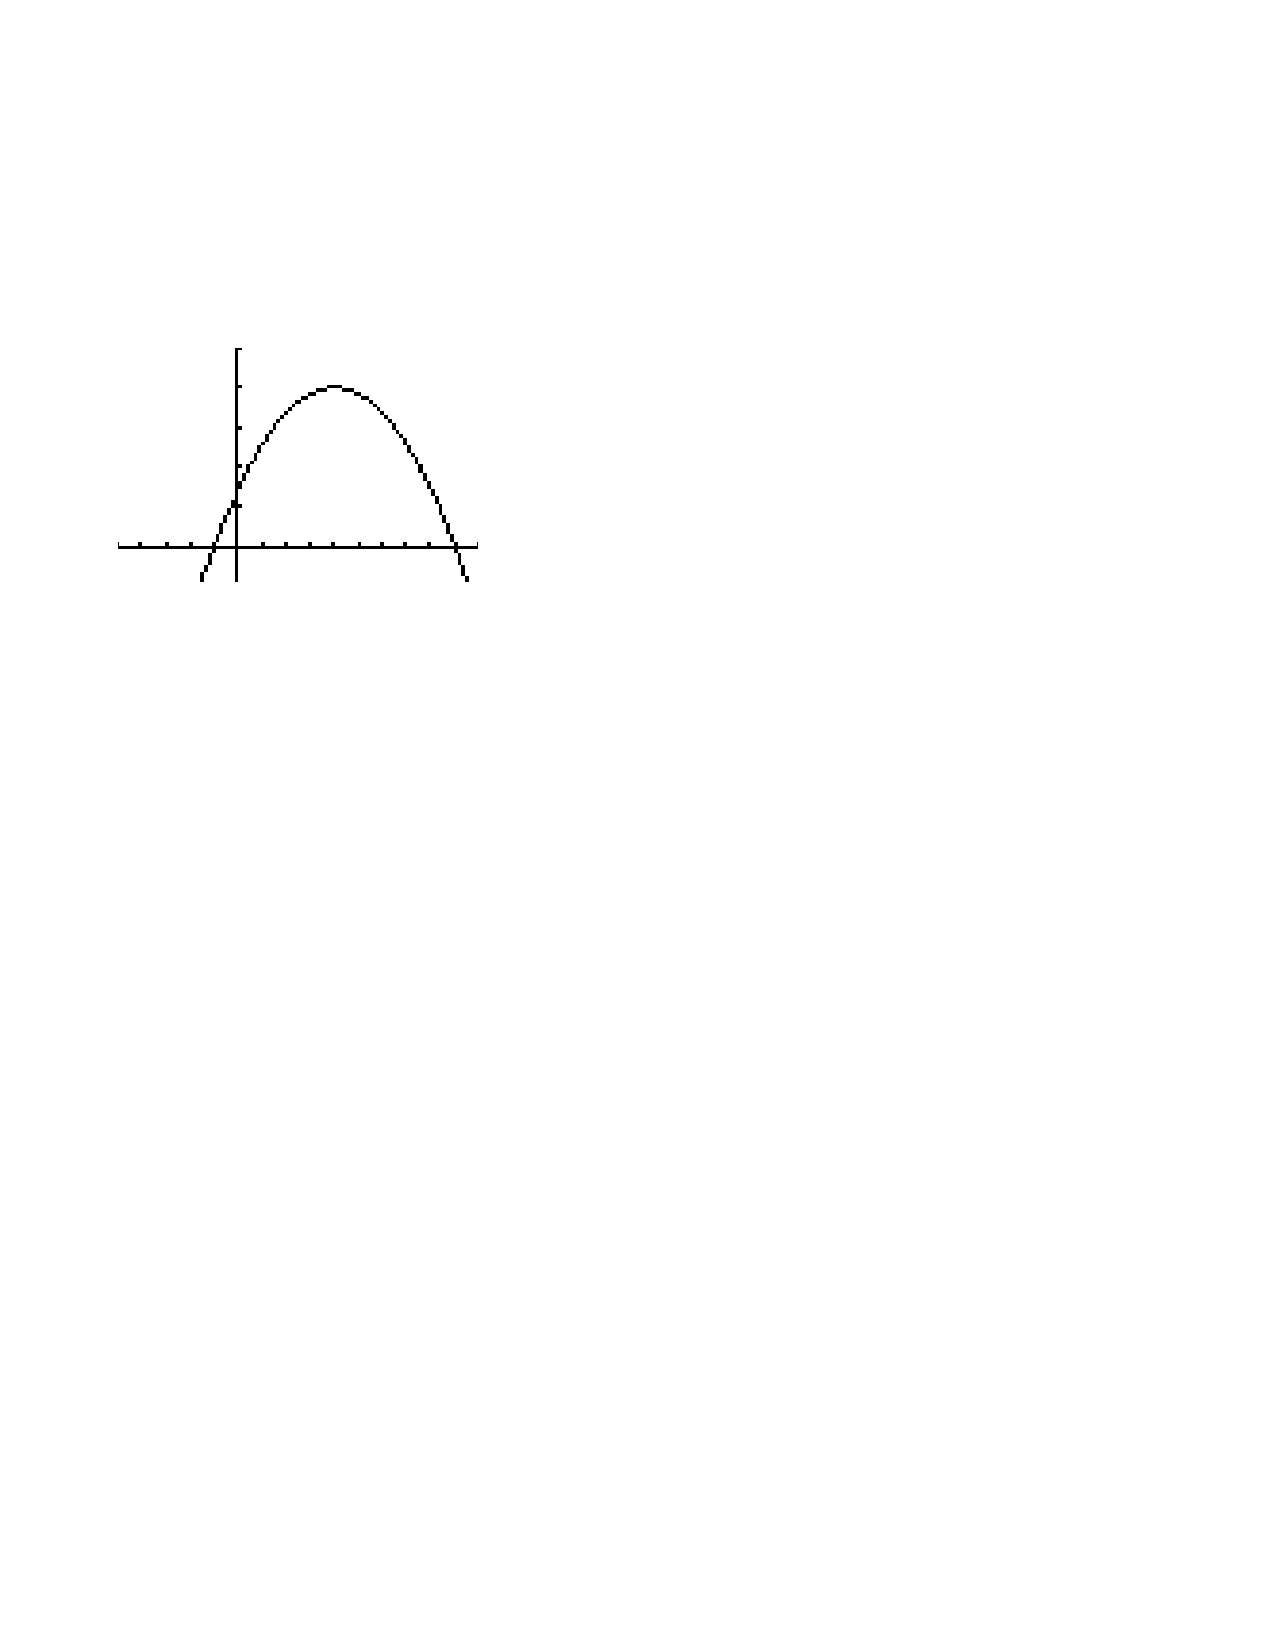
\includegraphics[scale=.7]{Figure4.pdf}
		\end{image}
		\end{freeResponse}

	\item Find the domain and range of $h$.
		\begin{freeResponse}
		The domain of $h(x)=ln(x)$ is $(0,\infty)$.  The range is $(-\infty,\infty)$.
		\end{freeResponse}

	\item Find the values of $h(1), h(0), h(-1), h(e), h\left(\frac{1}{e}\right)$, or say $x$ not in the domain.
			\begin{freeResponse}
			 $$h(1)=ln(1)=0$$
			$$ h(0)\ \text{is not defined}, 0\ \text{is not in the domain}$$
			$$ h(-1)\ \text{is not defined}, -1\ \text{is not in the domain}$$
			$$h(e)=ln(e)=1$$
			$$h\left(\frac{1}{e}\right)=\ln\left(\frac{1}{e}\right)=\ln\left(e^{-1}\right)= -1\ln(e)=-1$$
			 These are values of $h(x)=ln(x)$ that you should know.
		\end{freeResponse}
	\end{enumerate}
	
 		
		
	
\end{problem}




%problem 3
\begin{problem}
Given $y(t)=t- \frac{\pi}{3}$ and $w(t)=\sin(t)$.  Find:
\begin{enumerate}	
	\item  $y(w(t))$
		\begin{freeResponse}
			$y(w(t))=y\left( \sin(t) \right)=\sin(t)-\frac{\pi}{3}$
		\end{freeResponse}	


	\item  $w(y(t))$
		\begin{freeResponse}
		$w(y(t))=w\left( t-\frac{\pi}{3}\right)=\sin\left( t-\frac{\pi}{3}\right)$
		\end{freeResponse}	


	\item  $w \left(y \left(\frac{4\pi}{3} \right)\right)$
		\begin{freeResponse}
		$w \left(y \left(\frac{4\pi}{3} \right)\right)=\sin \left(\frac{4\pi}{3}-\frac{\pi}{3}\right)=sin(\pi)=0$
		\end{freeResponse}	


	\item  $y(w(\frac{4\pi}{3}))$
		\begin{freeResponse}
		$y \left(w \left(\frac{4\pi}{3} \right)\right)=\sin \left(\frac{4\pi}{3}\right)-\frac{\pi}{3}=\frac{-\sqrt{3}}{2}-\frac{\pi}{3}$

		You should know values of $sin(x)$ and $cos(x)$ for all values found on the standard unit circle.
		\end{freeResponse}	
	
	\end{enumerate}
	
	
\end{problem}



%problem 4
\begin{problem}
Define 
	$g(x) =   \left\{ \begin{array}{cl}
	|x-2|		 	&	\qquad \text{if } x < 0					\\
	\cos(x)			&	\qquad \text{if }  x \geq 0  	\\		\end{array} \right.  $
\begin{enumerate}	
	\item  Sketch a graph of $g$
		\begin{freeResponse} \hfil
			\begin{image}			
			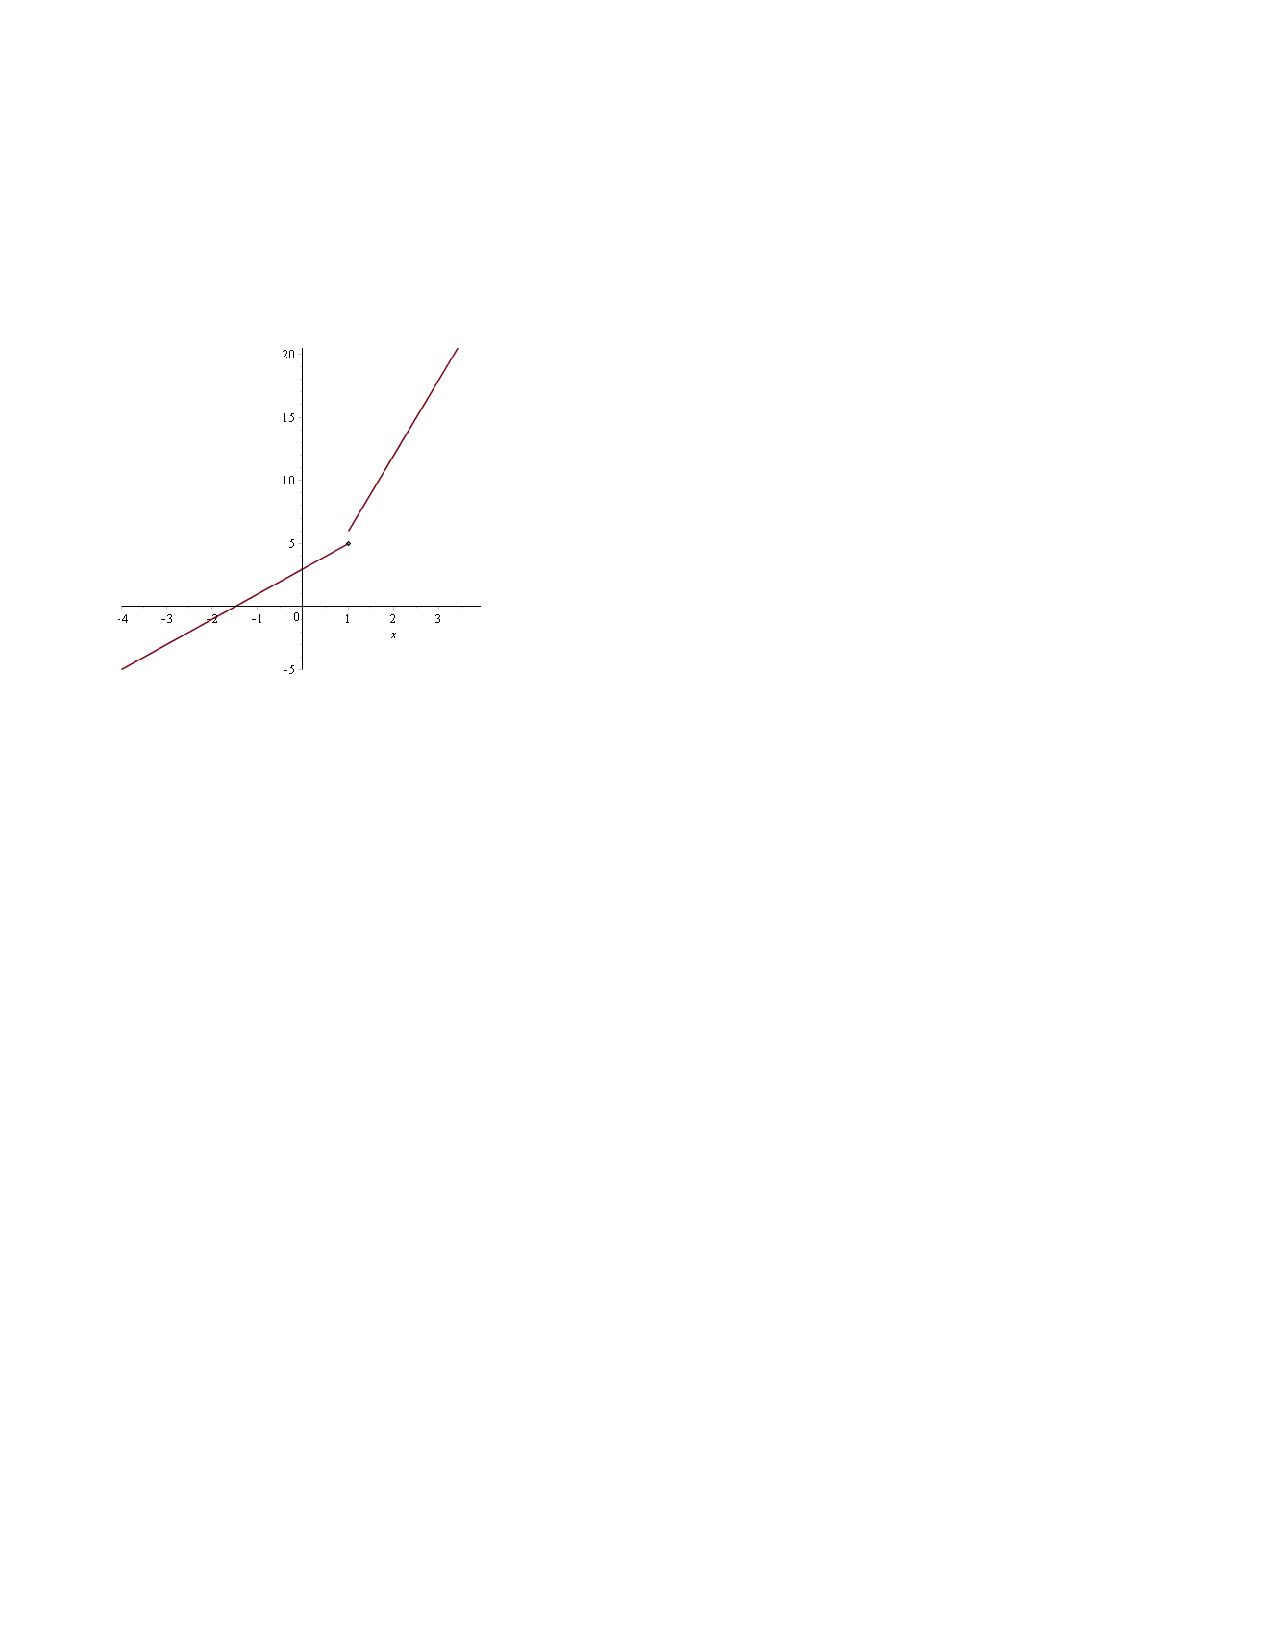
\includegraphics[scale=.7]{Figure6.pdf}
			\end{image}

		\end{freeResponse}

	\item  Find the domain and range of $g$
		\begin{freeResponse}	
			Domain: $(-\infty,\infty)$, Range: $[-1,1]\cup(2,\infty)$
		\end{freeResponse}		
	
	\item  Find the values of $g(\pi)$ and $g(-\pi)$
		\begin{freeResponse}	
			$g(\pi)=\cos (\pi)=-1$ and $g(-\pi)=|-\pi-2|=\pi+2$
		\end{freeResponse}
	
	\end{enumerate}

\end{problem}

%problem 5
\begin{problem}
The entire graph of $f(x)$ is given below.

	\begin{image}
	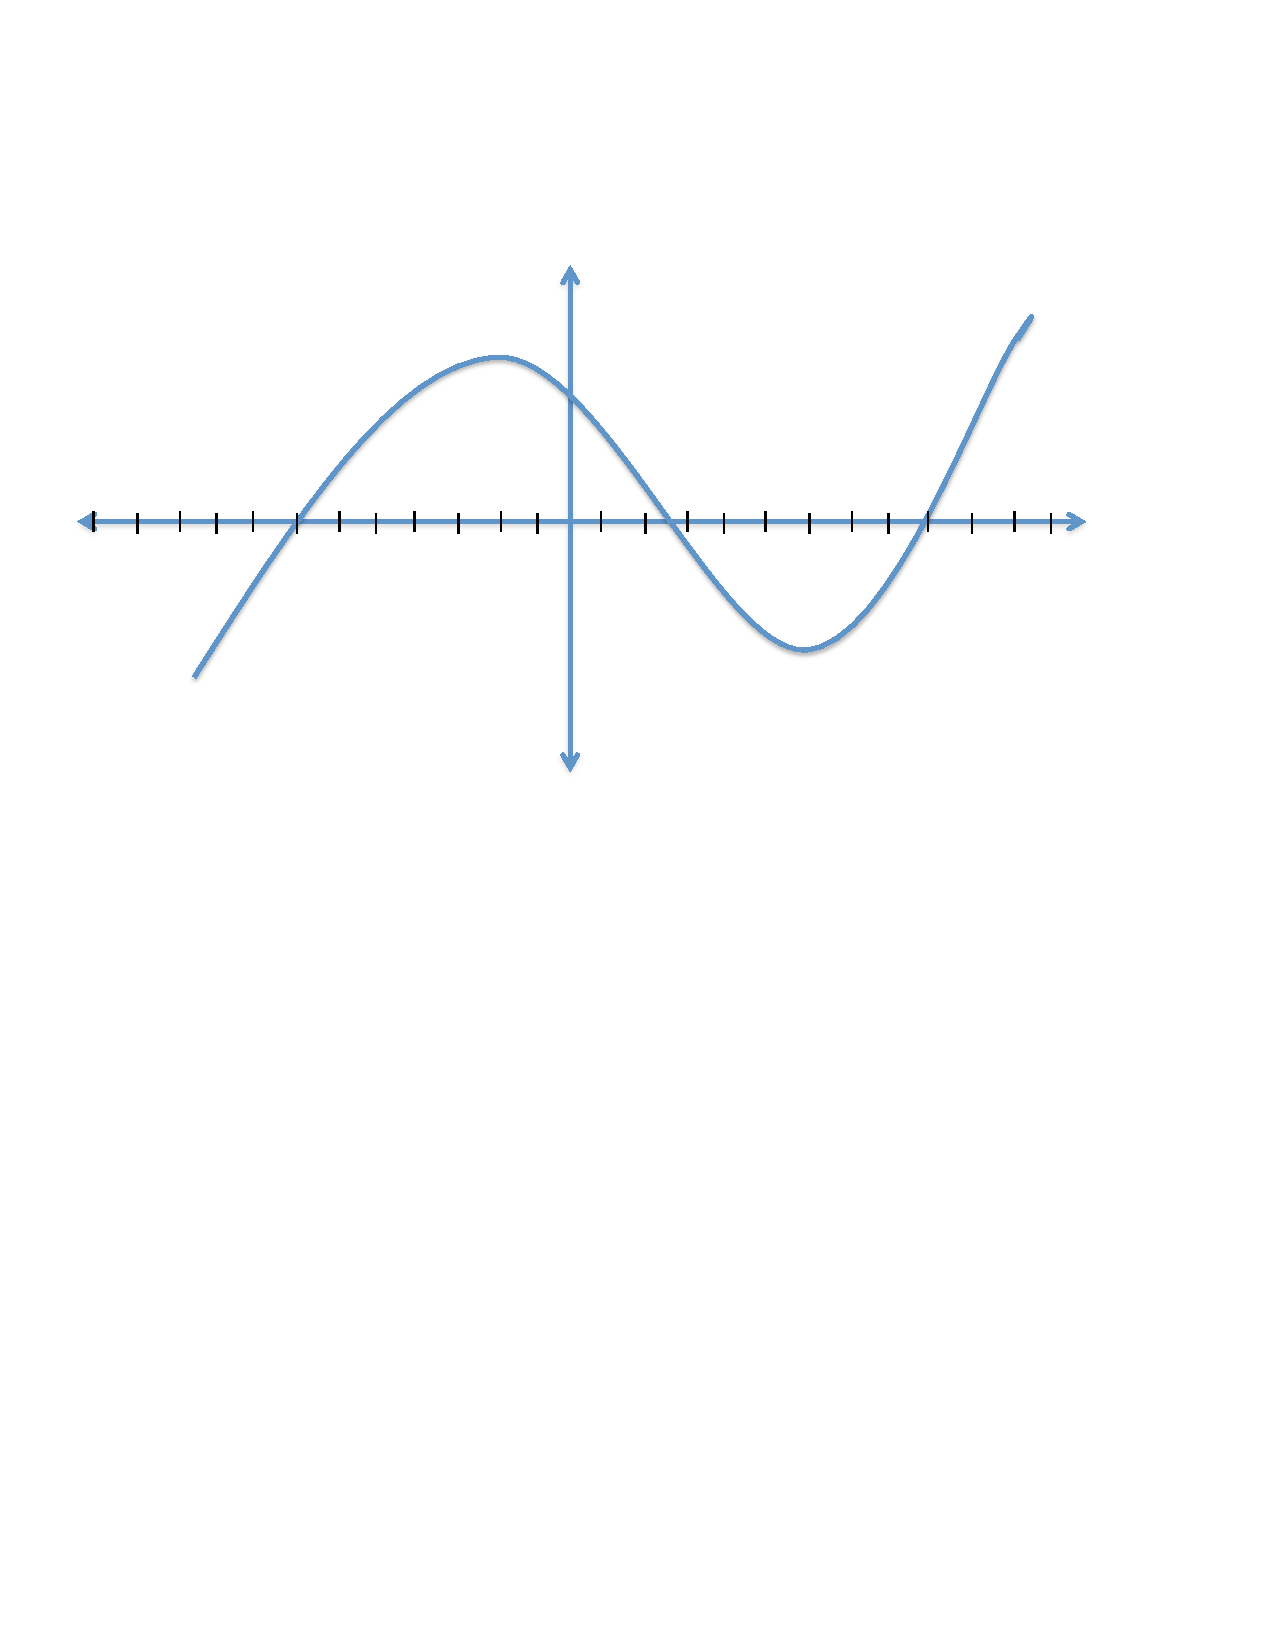
\includegraphics[scale=.8]{Figure2.pdf}
	\end{image}

\begin{enumerate}	
	\item  Find the domain and range of $f$
		\begin{freeResponse}
			Domain: $[-4,-3]\cup\left\{-2\right\}\cup(-1,4]$
			Range: $[-4,-3)\cup\left\{-2\right\}\cup[-1,3)$
		\end{freeResponse}	

	\item  Find the values of $f(-3),f(-2), f(-1),f(2)$
		\begin{freeResponse}
		$f(-3)=0, f(-2)=-2, f(-1)\ \text{does not exist}, f(2)=-1$
		\end{freeResponse}	

	\item  Find the intervals on which $f(x)$ is postive.  Find the intervals on which $f(x)$ is negative.
		\begin{freeResponse}
		 $f(x)$ is postive on $(1,2)$. $f(x)$ is negative on $[-4,-3),\left\{-2\right\},(-1,1),[2,4)$
		\end{freeResponse}
	
	\item Find the intervals on which $f$ is increasing.  Find the intervals on which $f$ is decreasing.
		\begin{freeResponse}
		$f$ is increasing on $(-4,-3),(0,2),(2,4)$.  $f$ is decreasing on $(-1,0)$
		\end{freeResponse}
	
	\item True or False: $f(1.5) < f(2)$
		\begin{freeResponse}
		False, $f(2) < f(1.5)$
		\end{freeResponse}	
	
	\end{enumerate}

	
\end{problem}



%problem 6
\begin{problem}
Determine if the function is even, odd, or neither.


\begin{enumerate}	
	\item  $h(x)=x^4+x^2-3$
		\begin{freeResponse}

		A function is even if $f(x)=f(-x)$, for all $x$ in the domain, which means its graph is symmetic about the y-axis.  A function is odd if $f(-x)=-f(x)$, for all $x$ in the domain, which means its graph is symmetic about the origin. 
		 $$h(x)=x^4+x^2-3$$
			$$h(-x)=(-x)^4+(-x)^2-3=x^4+x^2-3$$
			$h(x)=h(-x)$.  Hence $h$ is even.  This can be verified by graphing $h$ and seeing that its graph is symmetric about the y-axis.
		\end{freeResponse}

	\item  $s(t)=t^2-t$
		\begin{freeResponse}
			$$s(t)=t^2-t$$
			$$s(-t)=(-t)^2-(-t)=t^2+t$$ This does not equal $s(t)$ so $s(t)$ is not even.
			$$-s(t)=-(t^2-t)=-t^2+t$$  This does not equal $s(-t)$ so $s$ is not odd.  Hence, $s(t)$ is neither even, nor odd.
		\end{freeResponse}

	\item  We know that $\sin(\theta)$ is odd and $\cos(\theta)$ is even.  Is $g(\theta)=\tan(\theta)$ even, odd, or neither?
		\begin{freeResponse}
		 $$g(\theta)=\tan(\theta)=\frac{\sin(\theta)}{\cos(\theta)}$$
			\begin{align*}
			g(-\theta)&=\frac{\sin(-\theta)}{\cos(-\theta)}\\
			&=\frac{-\sin(\theta)}{\cos(\theta)}\\
			&=-\frac{\sin(\theta)}{\cos(\theta)}
			\end{align*}
			\begin{center}
			$$-g(\theta)=-\frac{\sin(\theta)}{\cos(\theta)}$$
			$g(-\theta)=-g(\theta) \implies g$ odd
			\end{center}
		\end{freeResponse}
	\end{enumerate}
	

	
\end{problem}




%problem7
\begin{problem}
Using the known graphs of $y=\sqrt{x}$ and $y=\frac{1}{x}$, sketch the graphs of the following using transformations.

\begin{enumerate}
 	\item $y=\sqrt{x+2}-3$
	\begin{freeResponse}
		This is a shift of $y=\sqrt{x}$ moved left 2 units and down three units.
	\begin{image}		
	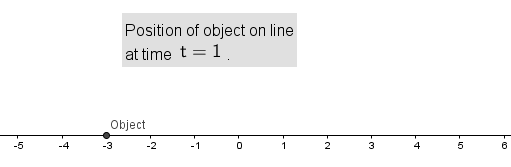
\includegraphics[scale = 0.7]{Figure8.png}
	\end{image}
	\end{freeResponse}
	

	\item $y=\frac{1}{x-4}+1$

	\begin{freeResponse}
		This is a shift of $y=\frac{1}{x}$ moved right 4 units and up one unit.
		\begin{image}		
	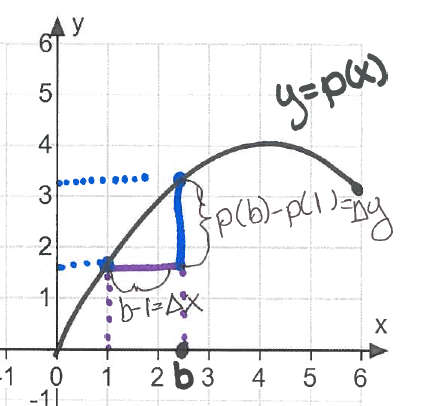
\includegraphics[scale=0.7]{Figure7.png}
	\end{image}
	\end{freeResponse}
\end{enumerate}

\end{problem}

%problem8
\begin{problem}
Find the domain of the function.  Determine whether the function is odd, even, or neither.

\begin{enumerate}
	\item $f(x)=\frac{x}{\sqrt{x^2-9}}$
		\begin{freeResponse}
			To find the domain, recall that a rational expression cannot have $0$ in the denominator and a square root expression cannot have a negative number under the square root.  Thus, $x^2-9>0$.
			$\implies (x-3)(x+3)>0$  The zeros are located at $x=-3,3$.  From this we can draw a sign chart  for the expression, $x^2-9$, and test values.
		\begin{image}		
	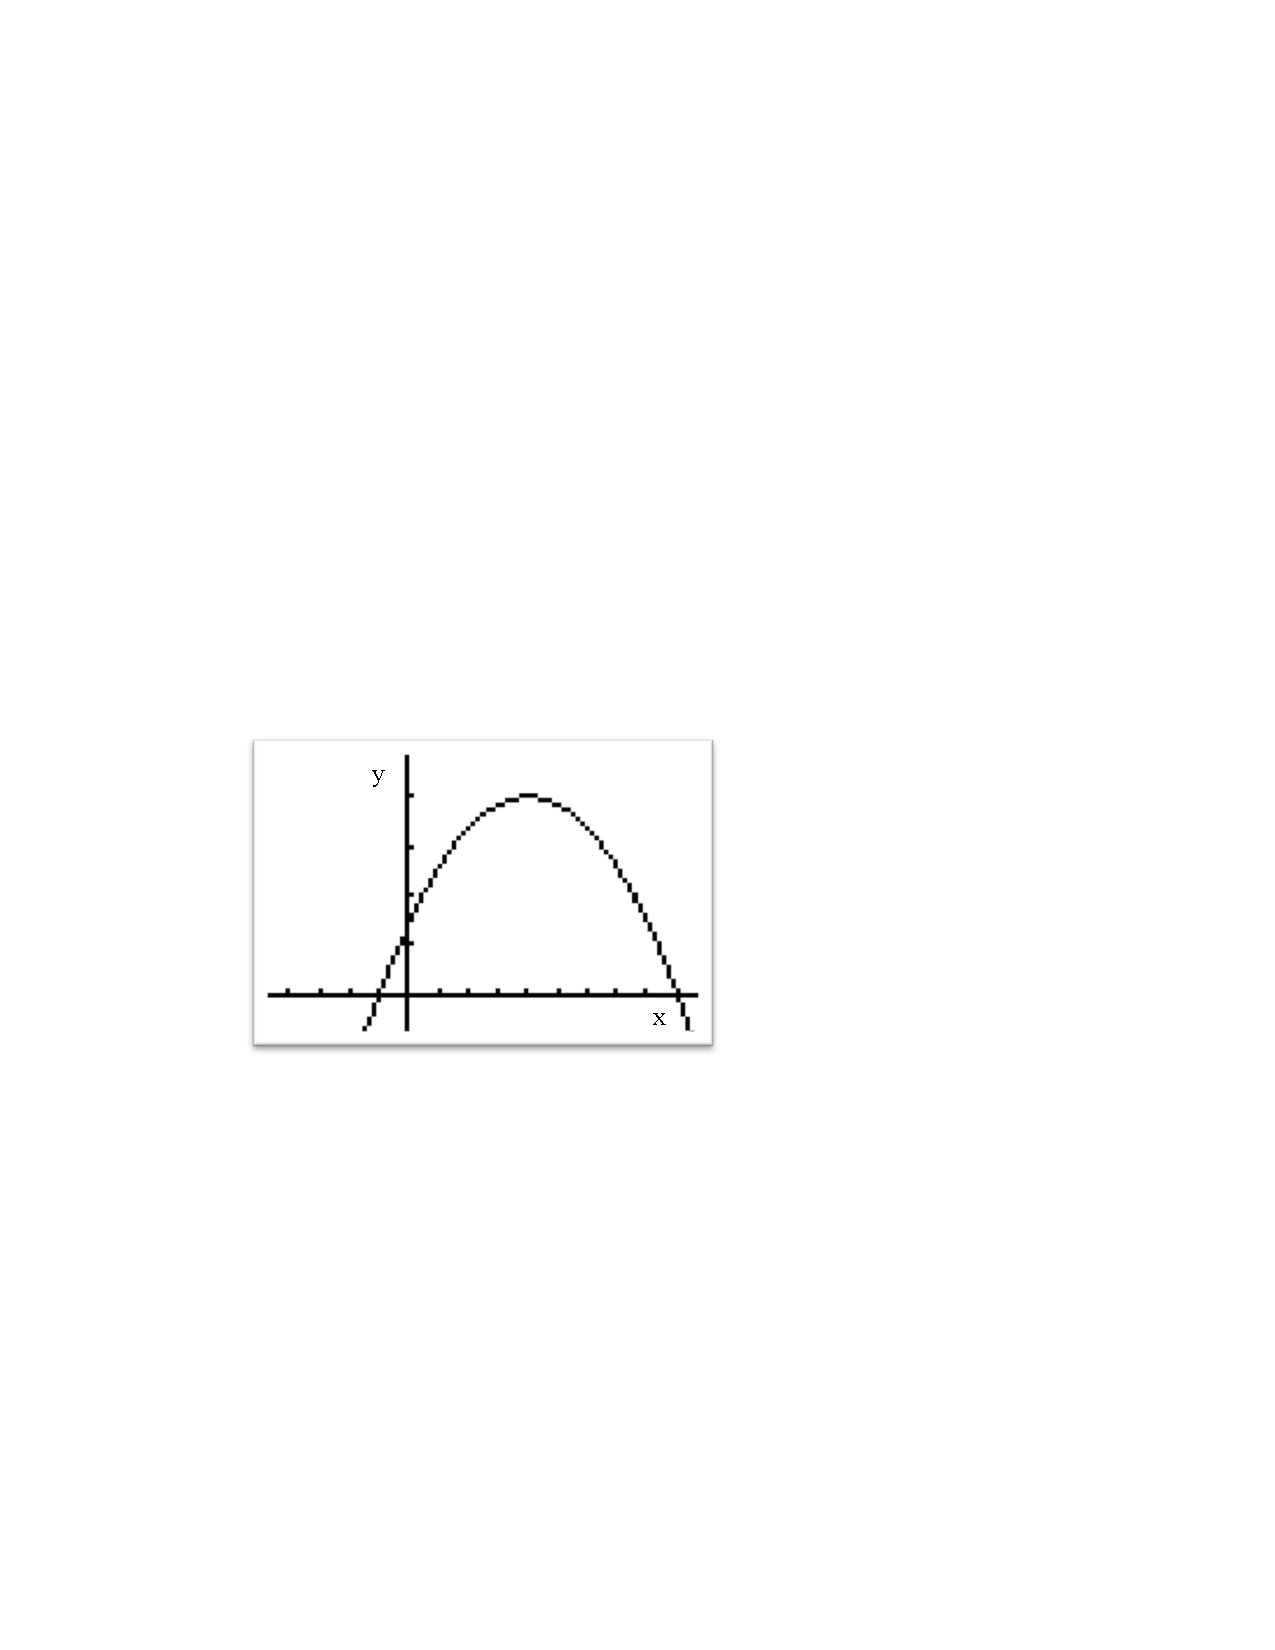
\includegraphics[scale=0.2]{Figure9.png}
	\end{image}
		We see that $x^2-9>0$ on the interval $(-\infty,-3)\cup (3,\infty)$.  Thus our domain is $(-\infty,-3)\cup (3,\infty)$.\\ \\

		Next we check for even/odd/neither.\\
		$f(-x)=\frac{-x}{\sqrt{(-x)^2-9}}$ which does not equal $f(x)$ so $f$ is not even\\
		$-f(x)=-\frac{x}{\sqrt{x^2-9}}$ which is equal to $f(-x)$ so $f$ is odd.
		
		\end{freeResponse}

	\item $g(x)= \frac{\sin(x)}{x}$
		\begin{freeResponse}
	To find the domain, recall that a rational expression cannot have $0$ in the denominator.  Therefore, our domain is $(-\infty,0) \cup (0,\infty)$\\ \\
	
	Next we check for even/odd/neither.\\
		$f(-x)= \frac{\sin(-x)}{-x}=\frac{-\sin(x)}{-x}=\frac{\sin(x)}{x}$ which equals $f(x)$ so $f$ is even


		\end{freeResponse}

	\item $h(t)= \ln(t^3-1)$

		\begin{freeResponse}
		To find the domain, recall that we cannot take the natural logarithm of $0$ or a negative number.  Therefore, $t^3-1>0$.
			$\implies (t-1)(t^2+t+1)>0$.  The zero is located at $t=1$.  From this we can draw a sign chart and test values.

	\begin{image}		
	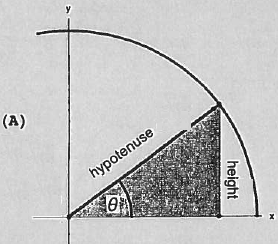
\includegraphics[scale=0.2]{Figure10.png}
	\end{image}
		We see that $t^3-1>0$ on the interval $(1,\infty)$.  Thus our domain is $ (1,\infty)$.\\ \\
		
		Next we check for even/odd/neither.\\
		$h(t)$ is neither even nor odd because if $t$ is in the domain, then $-t$ is not in the domain.


		\end{freeResponse}

\end{enumerate}

\end{problem}

%problem9
\begin{problem}
For any function $f$ defined on $(-\infty,\infty)$, we can define $f_e$ and $f_o$ as follows: $f_e=\frac{f(x)+f(-x)}{2}$ and $f_o=\frac{f(x)-f(-x)}{2}$


\begin{enumerate}	
	\item  Show  $f_e=\frac{f(x)+f(-x)}{2}$  is even
		\begin{freeResponse}	
			 $$f_e=\frac{f(x)+f(-x)}{2}$$
			We want to show this is an even function, so we need to show $f_e(-x)=f_e(x)$ for all $x$
			$$f_e(-x)=\frac{f(-x)+f(-(-x))}{2}$$ 
			$$=\frac{f(-x)+f(x)}{2}$$
			$$=f_e(x)$$
		\end{freeResponse}

	\item  Show $f_o=\frac{f(x)-f(-x)}{2}$ is odd
		\begin{freeResponse}	
			 $$f_o=\frac{f(x)-f(-x)}{2}$$
			We want to show this is an odd function, so we need to show $f_o(-x)=-f_o(x)$ for all $x$
			First, we'll find $-f_o$
			\begin{align*}
			-f_o(x)&=-\frac{f(x)-f(-x)}{2}
			\end{align*}

			Now we'll find $f_o(-x)$
			\begin{align*}
			f_o(-x)&=\frac{f(-x)-f(-(-x))}{2}\\
			&=\frac{f(-x)-f(x)}{2}\\
			&=-\frac{f(x)-f(-x)}{2}\\
			&=-f_o(x)
			\end{align*}
			
		\end{freeResponse}
	\item Show that $f(x)=f_e(x)+f_o(x)$, for all $x$
		\begin{freeResponse}
		
		We want to show that $f(x)=f_e(x)+f_o(x)$, for all $x$.  From parts a and b, we know $f_e=\frac{f(x)+f(-x)}{2}$ and $f_o=\frac{f(x)-f(-x)}{2}$.  Therefore,
			\begin{align*}
			f_e(x)+f_o(x)&=\frac{f(x)+f(-x)}{2}+\frac{f(x)-f(-x)}{2}\\
			&=\frac{f(x)+f(-x)+f(x)-f(-x)}{2}\\
			&=\frac{2f(x)}{2}\\
			&=f(x)
			\end{align*}
		We have just proved that every function defined on $(-\infty,\infty)$ can be written as the sum of an odd function and an even function.
	
		\end{freeResponse}

	\item Is there a function that is both even and odd?
		\begin{freeResponse}
		$f(x)=0$ is both even and odd because $f(x)=f(-x)=0$ for all $x$ and $-f(x)=f(-x)=0$ for all $x$
		\end{freeResponse}

	\item Something to think about:  Write each function as an even function plus an odd function.
	
	\begin{enumerate}
		\item $f(x)=\sin(x)$
			\begin{freeResponse}
				$f_e(x)=0$ and $f_o(x)=\sin(x)$.  $f(x)=0+\sin(x)$

			\end{freeResponse}
				\item $f(x)=x^3+2x^2+x$
			\begin{freeResponse}
				$f_e(x)=2x^2$ and $f_o(x)=x^3+x$.  $f(x)=2x^2+x^3+x$

			\end{freeResponse}
				\item $f(x)=\ln(x)$
			\begin{freeResponse}
				$f(x)=\ln(x)$ is not defined on $(-\infty,\infty)$.  It is only defined on $(0,\infty)$.  It doesn't make sense to think about the natural logarithm as even or odd.
			\end{freeResponse}
				\item $f(x)=e^x$
			\begin{freeResponse}
				$f_e(x)=\frac{f(x)+f(-x)}{2}=\frac{e^x+e^{-x}}{2}$ and $f_o(x=\frac{f(x)-f(-x)}{2})=\frac{e^x-e^{-x}}{2}$.  \\\\
				$f(x)=\frac{e^x+e^{-x}}{2}+\frac{e^x-e^{-x}}{2}$

			\end{freeResponse}	

	\end{enumerate}
	\end{enumerate}
	

\end{problem}
\end{document} 









